\documentclass[]{homework}
\usepackage{multirow}
\usepackage{graphicx}
\usepackage{tikz}
\usepackage{amsmath}	% math fonts
\usepackage{amsthm}
\usepackage{amsfonts}

\usetikzlibrary{arrows,automata}
\usetikzlibrary{decorations.pathmorphing} % noisy shapes
\usetikzlibrary{fit}					% fitting shapes to coordinates
\usetikzlibrary{backgrounds}	% drawing the background after the foreground

\begin{document}
\header{CS5340}{Project Proposal}{Shawn Tan \& Davin Choo}

\section{Introduction}
With more user-generated content appearing online, it is useful to be able to
extract data from sites with user-created content in a timely manner. A naive
way of getting timely updates is to aggressively fetch the pages repeatedly,
downloading the pages at a frequent rate. However, the number of pages in a
forum site are far too large to perform this efficiently on every forum. One
way to minimise this cost would be to look at the time differences between
previous posts to estimate the arrival of the next one. A possible improvement
would be to see if we can use the content of the posts to make a guess as to
when the next post will arrive. In this project, our goal is to predict updates
in forum threads, based on the content of previous posts.

We plan to use Hidden Markov Models (HMM) to model the thread update behaviour, 
using it and observations made from the content of the previous posts to then 
predict what the expected time of the next post arrival will be. For our dataset 
we extracted the timestamp, author and text content for each post in each thread 
from the forums.  Our dataset was obtained from \url{http://www.avsforum.com}.  
This forum was chosen due to the better standard of English used, allowing for 
methods of natural language to be applied such as stemming.

In Section \ref{prop_method} we provide a detailed description of the model we 
use for our project, along with how we will obtain the various parameters to 
create the HMM. We then provide a proposed timeline in Section \ref{prop_plan}, 
which will provide a rough schedule of when various milestones of the project 
will be achieved.

\section{Proposed Method}\label{prop_method}

We use a windowing method to obtain instances from our dataset. A window of size 
$w$ will be considered at each time step, and observations, namely the word 
frequencies and the time differences within the window will be considered.

\begin{figure}[h]
	\begin{center}
		\tikzstyle{state}=[circle,
	thick,
	minimum size=1.2cm,
	draw=blue!80,
	fill=blue!20]
% The measurement vector is represented by an orange circle.
\tikzstyle{measurement}=[circle,
	thick,
	minimum size=1.2cm,
	draw=orange!80,
	fill=orange!25]

\tikzstyle{background}=[rectangle,
	fill=gray!10,
	inner sep=0.2cm,
	rounded corners=5mm]

\begin{tikzpicture}[>=latex,text height=1.5ex,text depth=0.25ex]
    % "text height" and "text depth" are required to vertically
    % align the labels with and without indices.
  
  % The various elements are conveniently placed using a matrix:
  \matrix[row sep=2cm,column sep=0.3cm] {
    % First line: Control input
    	&
		\node (prev_state)					{$\cdots$};&
		&
        &
        \node (curr_state)	[state]			{$q_t$}; &
        &
		&
		\node (next_state)					{$\cdots$};&
		&
        \\
		&
		&
		\node (obs_text)	[measurement]	{$\Delta_t$};&
		&
		&
		&
		\node (obs_time)	[measurement]	{$\mathbf{v}$};&
		&
        \\
	};
    
    % The diagram elements are now connected through arrows:

	\path[->]
		(prev_state) edge[thick]	(curr_state)
		(curr_state) edge[thick]	(next_state)
		(curr_state) edge			(obs_text)
		(curr_state) edge			(obs_time)
	;
 	  \begin{pgfonlayer}{background}
        \node [background,
					fit=\onslide<1>{(prev_state) (next_state)},
                    label=left:Hidden states:] {};
    \end{pgfonlayer}
\end{tikzpicture}

	\end{center}
	\caption{Observations and transitions per state.}\label{per_state}
\end{figure}

Figure \ref{per_state} illustrates the Hidden Markov Model we plan to model the 
behaviour of replies on forum threads with. Each state emits different 
frequencies of words, which are represented with $\mathbf{v}$, and have 
different distributions of time intervals, represented with $\Delta_t$.

The intuition behind the modelling of the system in this manner is that there is 
some state governing the behaviour of the thread posts. Active threads can 
transition to an inactive state, but the presence of a new post is able to spark 
off a new discussion within the thread, causing it to be an active thread again.
It remains now to determine what these states are, and what the probabilities of 
the state transitions are.

A simplistic model of how this model could work would be a two-state HMM. In 
this case, the states, say $q_1$ and $q_2$, could represent an `active' thread, 
and an `less active' thread, with the mean $\Delta_t$ (time intervals between 
posts) being, say, 6 minutes and 240 minutes respectively.

Using a simple Naive Bayes classifier, we could obtain 
$\P{q_i}{\Delta_t,\mathbf{v}}$, and the state transitions $\P{q_t}{q_{t-1}}$	
could be learnt from the dataset by counting. With these in place, we can then 
observe the posts in sequence, and then update the distribution of which state 
we are currently in appropriately. We would also need to attach an average time 
for next post per state. This would then allow us to calculate the expected time 
for the arrival of the next post. Figure \ref{spaceship} illustrates this simple 
example.

\begin{figure}
	\begin{center}
		\tikzstyle{state}=[circle,
	thick,
	minimum size=1.2cm,
	draw=blue!80,
	fill=blue!20]


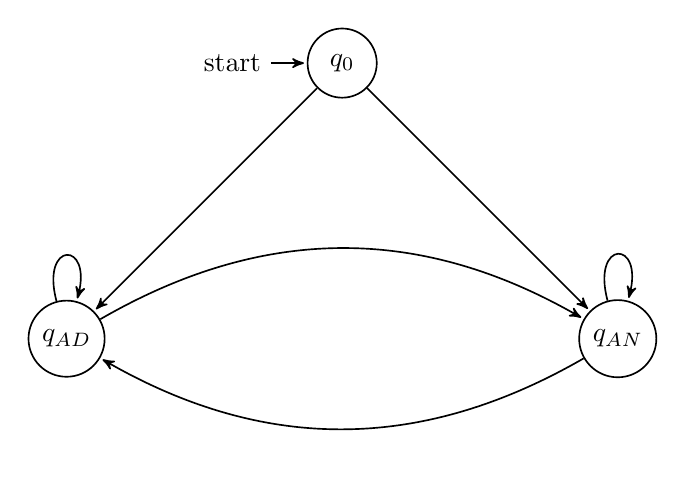
\begin{tikzpicture}[->,>=stealth',shorten >=1pt,auto,node distance=3.5cm,
                    semithick]

  \node[initial,state] (q0)                    {$q_0$};
%  \node[state]         (IN) [below of=q0] {$q_I$};
  \node[state]         (AD) [below of=q0, left of=q0] {$q_{AD}$};
  \node[state]         (AN) [below of=q0, right of=q0] {$q_{AN}$};

  \path (q0) edge              node {} (AD)
 			 edge 			   node {} (AN)
		(AD) edge [loop above] node {}(AD)
			 edge [bend left]  node {}(AN)
		(AN) edge [bend left]  node {}(AD)
			 edge [loop above] node {}(AN);
\end{tikzpicture}



	\end{center}
	\caption{Preliminary modelling of a thread as a probabilistic 
	automaton}\label{spaceship}
\end{figure}


\section{Proposed Plan}\label{prop_plan}

\begin{description}
	\item[Extracting Data, Preliminary Work]
Some work has already been done prior to the submission of this proposal.  
Statistics for the state transitions and the word frequencies produced in each 
state have been collected.  A plot of the probability density can be seen in 
Figure \ref{dplot}.  The plot shows a sample of the transition probabilities if 
the time intervals were binned into 20 minute blocks, and each of these bins 
were used as a state.  Here, we show only up to bin 100, but we can still see 
that forum posts rarely go from a short time interval to a long time interval.  
Posts which have a long time interval, however, tend to go back to having short 
time intervals.

\begin{figure}
	\begin{center}
		\includegraphics[scale=0.7]{figure_1.png}
	\end{center}
	\caption{Probability density matrix plot for 
	$\P{q_{t+1}}{q_t}$}\label{dplot}
\end{figure}
	\item[Learning the Parameters]
A probability distribution function of the time intervals has to be estimated, 
using the same distribution found in Kleinberg's model \cite{Kleinberg2003}
using HMMs for classifying emails into a hierarchical structure.
One possibility we could be exploring would also be to cluster the posts 
according to some topics using Latent Dirichlet Allocation, and then taking the 
average time intervals for each of the topics. The topics could then be 
represented as states, and the transitions between these states learnt from the 
data.
	\item[Possible Improvements]
Considering a crawler that uses this prediction method to revisit pages, one 
would find that mistakes may be made: The crawler visits too early, and wastes a 
page download. The crawler could also visit the page after two posts, which 
takes a toll on the freshness of the database it is maintaining. One possible 
improvement we could make would be to update the state distribution when we make 
a visit and do not get anything new. We could also update the transition 
probabilities whenever we observe new posts, making the system adaptive to 
changes in the posting behaviour of the site.

\end{description}
\bibliographystyle{acm}
\bibliography{proposal}
\end{document}
